
%%%%%%%%%%%%%%
%%% DESIGN %%%
%%%%%%%%%%%%%%

\chapter{Design}

The thesis investigated here is that using tabletops as basic IO peripherals for other computing devices will help their adoption by the public.
A user should be able to transfer the display of his/her device to a tabletop, and interact with it in a natural way.
The success of such an interaction model depends on the usability of the system. 

To avoid any confusion, a few concepts must be defined.
The system involves a \emph{person}, a \emph{personal device} and a \emph{tabletop}.
Human computer interaction takes place on the screen of the tabletop.
The application UI is divided in two main parts.
The \emph{display extension}, or \emph{remote UI}, is a window that replicates the display of the personal device on the tabletop, relaying touch input and graphical output dynamically.
The \emph{surface UI} consists of UI elements on the tabletop that allows the manipulation and control of the remote UI on the interactive surface.

This chapter presents the design process of such a system.
Section 1 focuses on understanding the context of use and section 2 is an analysis of the requirements. Together they present the conceptual design.
Section 3, 4, and 5 describe the process of realizing a physical design for the surface UI element. They respectively present the generation of ideas, their evaluation through a participatory usability study, and the design decisions.

\section{Enhancing mobile computing with tabletops}
% (understanding the application context)

It is critical to understand fully the context in which the system will be used in order to achieve a good design.
Most users own a computing device with personal data and applications that are tailored to their needs.
Those personal devices are becoming smaller and more mobile, with devices such as tablet and handheld computers.
In many cases, the display size of the personal device is a limitation in terms of graphical input and output, and has a negative influence on the user experience.
One of the main characteristics of tabletops, however, is that they have superior graphical I/O capabilities.
This project focuses on situations where a tabletop can be used as a display extension to the personal device, thus enhancing the user experience.

Figure \ref{fig:useCase} describes the primary use case.
The system should basically be a graphical peripheral unit for other computing devices. Its main functions are to forward user input to the device, and to display graphical output from the device.

\begin{figure}[htb]
  \centering
    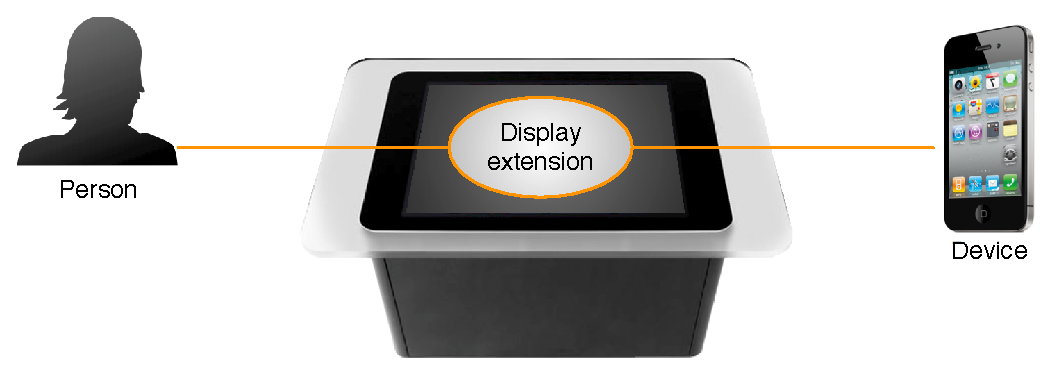
\includegraphics[width=0.9\textwidth]{images/useCase}
    \caption{Main use case.}
    \label{fig:useCase}
\end{figure}

\subsection{The devices}

\subsubsection{Tabletops}

A tabletop presents a range of characteristics that have concrete implications on the system design.
A tabletop is \ldots
\begin{description}

\item[\ldots a computer.] This project investigates a strategy where a tabletop is used as a smart IO peripheral.
The system should allow a tabletop to function as a relay between a personal device and users, forwarding both input and output as required.

\item[\ldots a table.] Its working surface is horizontal by nature, with the implication that it cannot support any prolonged interaction, because of the bad ergonomics of the ``hunched over'' working position.
Furthermore, a table gives naturally rise to various activities, such as eating, and it supports all sorts of objects, often in a collocated collaborative atmosphere.
The system should therefore support simultaneous users, and handle limited space availability.
Finally, a table offers no specific orientation, implying that the orientation of the system UI will have to adapt to the user's position around the tabletop.

\item[\ldots a situated device.] A tabletop is not mobile.
It usually sits at a specific location, and users come to it in order to use it.
The main implication is that tabletops seem to naturally fit in public spaces, where they are shared among multiple users.
This tendency is accentuated by the price factor, that makes a private person not likely to buy such a device for private use.
The system should handle public use, characterized by short anonymous sessions and an often interrupted interaction flow.
Other scenarios should be considered as well, such as a tabletop in an individual office, or in a family home.
In any case, it can be expected to have dedicated power supply and network connection, removing such concerns from the developer's mind.

\item[\ldots a shared device.] In many cases the tabletop will be shared by multiple users, raising concerns of user identification and data protection.

\item[\ldots an interactive surface.] As such, it typically offers large graphical output, as well as a range of input techniques to allow for user interaction.
Most tabletops support multitouch-based input.
This introduces a new kind of interaction model, more intuitive, that the system should be based upon.
In some cases, such as with camera-based devices, it is possible to add tangible objects to the tabletop experience.
This project reports on the possibilities to use a personal device as a tangible control integrated to the tabletop.

\end{description}

\subsubsection{Mobile computing devices}

A mobile computing device is \ldots

\begin{description}

\item[\ldots a computer.] It offers enough computing power, storage space and connectivity to support most users' daily tasks. The system should allow the user to access his/her applications and personal data.

\item[\ldots a small device.] Hence the mobility. Such a device is carried around by users. However, the small form factor implies a suboptimal graphical user experience.
The system should try to improve this, by offering superior IO resources.

\item[\ldots a mobile device.] With the implications that its power supply is limited by battery life, and its connectivity is unstable. The system should be developed with those concerns in mind.

\item[\ldots an interactive device.] Most mobile devices are now equipped with touch-based displays, making them naturally suitable for display extension on a tabletop.
However, all devices present physical buttons to the user as well.
The physical buttons implement strategic functions that the system should support.

\end{description}

\subsection{The situations}
\label{sec:scenarios}

There exists different types of everyday situations in which the system can be put to use.
They vary depending on whether they involve one or more users, and whether the tabletop is a public or private device.
A tabletop is considered a public device as soon as there are more than one user that have access to it.
As a consequence, the scenario of multiple users on a private tabletop is not considered.
Each situation implies a slightly different set of application features.
The original scenarios are included in appendix \ref{scenarios}.

\subsubsection{Single user on a public tabletop}

It should be possible for the user to wirelessly pair his/her personal device with a public tabletop computer.
This implies that the devices are both connected to the local wireless networks, that they are able to detect each other and discover each other's identity on the network.
It would not be safe to establish this connection automatically in a public space.
Therefore, dialogs should be used both on the mobile device and on the tabletop to gather user input.
The UI of the mobile device should be transferred to the interactive surface as graphical output, and this transferred display should be able to accept touch input to be forwarded back to the device.
The transferred display should be contained in an application window, and this window should be manipulable (drag, resize, rotate, minimize, hide, ..).

The application window should react to the state of the interactive surface.
An example of this is that the application window should turn inactive if it is obstructed by an object on the table.

Finally, the mobile device could be a participant in the interaction model, i.e. listing it off the table should interrupt the connection and exit the application.

%\begin{itemize}
%\item{the mobile device is automatically detected by the tabletop}
%\item{dialog windows are displayed on both devices}
%\item{the wireless connection is automatic}
%\item{the mobile device UI is transferred to the surface.}
%\item{the transferred UI can be resized, rotated and moved on the surface}
%\item{the transferred UI goes inactive when objects obstruct it}
%\item{user input is forwarded to the mobile device}
%\item{the transferred UI can be minimized and restored}
%\item{the application can be exited by lifting the mobile device off the table.}
%\end{itemize}

\subsubsection{Multi users on a public tabletop}

In a collocated collaborative context, it should be possible for more than one personal device to simultaneously have their display extended to the interactive surface.
This implies that the implementation should support parallel connections and simultaneous use.

Mobile computing devices come in many forms, and ideally the system should support all of them.
Devices vary in terms of software and hardware specifications.
Some parameters that are especially important here are the programming platform, as well as the display resolution.

When a tabletop is used simultaneously by multiple users, there is a very concrete risk of lack of space on the surface.
This fact introduces a new need for the system, to allow a user to remove his/her personal device from the table, while keeping the display extension active.

\subsubsection{Single user on a private tabletop}

If the tabletop is private, such as a home computer or a working desk, the system should offer extended functionalities to the user.
He/she should have the option to configure the tabletop in order to allow/initiate those extended functionalities.
Some suggested functionalities are:
\begin{itemize}
\item automatic launch of the display extension application
\item push application widgets from the extended display to the tabletop
\item share data between the personal device and the tabletop
\end{itemize}

\section{Solution requirements}

The general focus is on a seamless user experience.

\subsection{Pairing}

%Establishing a connection between the devices with a cable has several limitations.
%It requires having the correct cable and localizing the connector on the device. The number of connectors is a limitation, as well as the length of the cable. MORE

Connecting a personal device to a tabletop should be a quick and easy process.
The system should include a detection mechanism that would allow the devices to become aware of each other, as well as a discovery protocol to gather the information necessary to the pairing, such as a Network IP.
The connection should be wireless to guarantee a smooth experience.
However, a public tabletop should not be allowed to gather data from, let alone connect to, a personal device without the explicit consent of its owner.
In the case of a trusted setup, it should be possible to bypass any explicit user input.
Exiting the application and closing the connection should also be easy, allowing the system to handle short successive sessions.

\subsection{Remote UI}

At the core of the system is the display extension.
The UI of the personal device should be transferred to the tabletop, allowing the user to interact with it in a natural way.
Graphical output from the personal device should be forwarded to the tabletop, and touch-based input from the tabletop should be forwarded to the personal device.

\subsection{Surface UI}

The user experience should be improved by using the display extension on the surface.
Therefore, it is important to provide for a rich interaction.
The transferred UI should be contained within a manipulable window on the tabletop.
Specifically, the user should be able to move, rotate and resize the window; as well as minimize, hide and restore it.
The system should include UI elements that implement the functions supported by the physical controls present on the personal device.
Those elements and their function should be obvious to the user.

%secondary features
Modern smartphones include sensors that allow to switch the display orientation by tilting the device.
This feature is strategic to certain applications, and should be implemented by the system.
Obviously, tilting the tabletop is unfeasible, so another solution is necessary.

As mentioned earlier, a tabletop's screen space would typically be shared among different applications and/or objects.
Therefore, the system should handle limited screen space, and obstruction of the display extension.

In a trusted setting, the user should have the possibility to push application widgets from the personal device to the tabletop, outside of the display extension, thus saving space on the latter.

\subsection{Tangible UI}

It is a natural thing to place an object on a table, and tabletops are designed to allow for the integration of physical artifacts.
Therefore, it should be possible to use the personal device as a tangible UI.
For example, it would seem obvious that placing the device on the tabletop would launch the pairing process, or that lifting it off would interrupt the connection.
Furthermore, it should be possible to control the position of the display extension by sliding the personal device on the surface.

\section{Interaction design: the surface UI}
\label{sec:interaction}

The solution requirements are divided into 4 elements: pairing procedure, remote UI, surface UI and tangible UI.
The rest of this chapter investigates the physical design of the surface UI only, for the following reasons.

The pairing procedure does not introduce anything new to the field. There are known solutions to this challenge, which are described in section \ref{}.
The remote UI replicates the UI of the personal device on the tabletop, and does not require any supplementary design.
Using the personal device as a tangible UI for the display extension raises a series of design and implementation challenges. It is the opinion of the author that this research angle is promising, but it was decided to leave it out of the project for reasons of time constraints.
\hfill\\
The surface UI is the part of the system that allows the user to manipulate the remote UI on the tabletop using touch-based input.
Touch-based interaction removes the necessity of having input peripherals such as keyboard and mouse, and provides the user with a more direct and sensual experience.
The aim is to achieve a design that allow the user interaction to be intuitive. 

\subsection{Generating ideas}

The generation of ideas is an important part of the design process.
David Benyon refers to it as envisionment \citep{Benyon:2010}, and defines it as the process of externalizing design thoughts.
The techniques that were used to permit this process are brainstorming, sketching, storyboarding and prototyping.

\subsubsection{Storyboards}

The scenarios mentioned in section~\ref{sec:scenarios} are used as a base for the making of storyboards.
Storyboarding helps getting a feeling for the general flow of the interaction with the system.
At the same time, it gives a visual dimension to the definition of the different system features, and raises new design issues.

Several system features were described in the scenario as being the effect of a tap on a button.
When storyboarding, it became obvious that having too many UI buttons would be cumbersome, which lead to the consideration of other interaction techniques.
Similarly, the challenge of the location and size of the display extension on application launch became apparent with the first storyboard.

\subsubsection{Low fidelity prototypes}

Paper prototypes were used to aid the process of generating and evaluating as many possible design solutions as possible.
Screenshots of the iPhone UI \citep{iphone} were printed out in various sizes, and used on a normal table to simulate interaction with the surface UI.
Figure \ref{paperProt} shows some prototypes and a working session.

\begin{figure}[htb]
  \centering
    \includegraphics[width=1\textwidth]{images/paperProtDouble}
  \caption{Working with low fidelity prototypes.}
  \label{paperProt}
\end{figure}

%\begin{figure}[h!]
%  \caption{Low fidelity prototypes.}
%  \centering
%    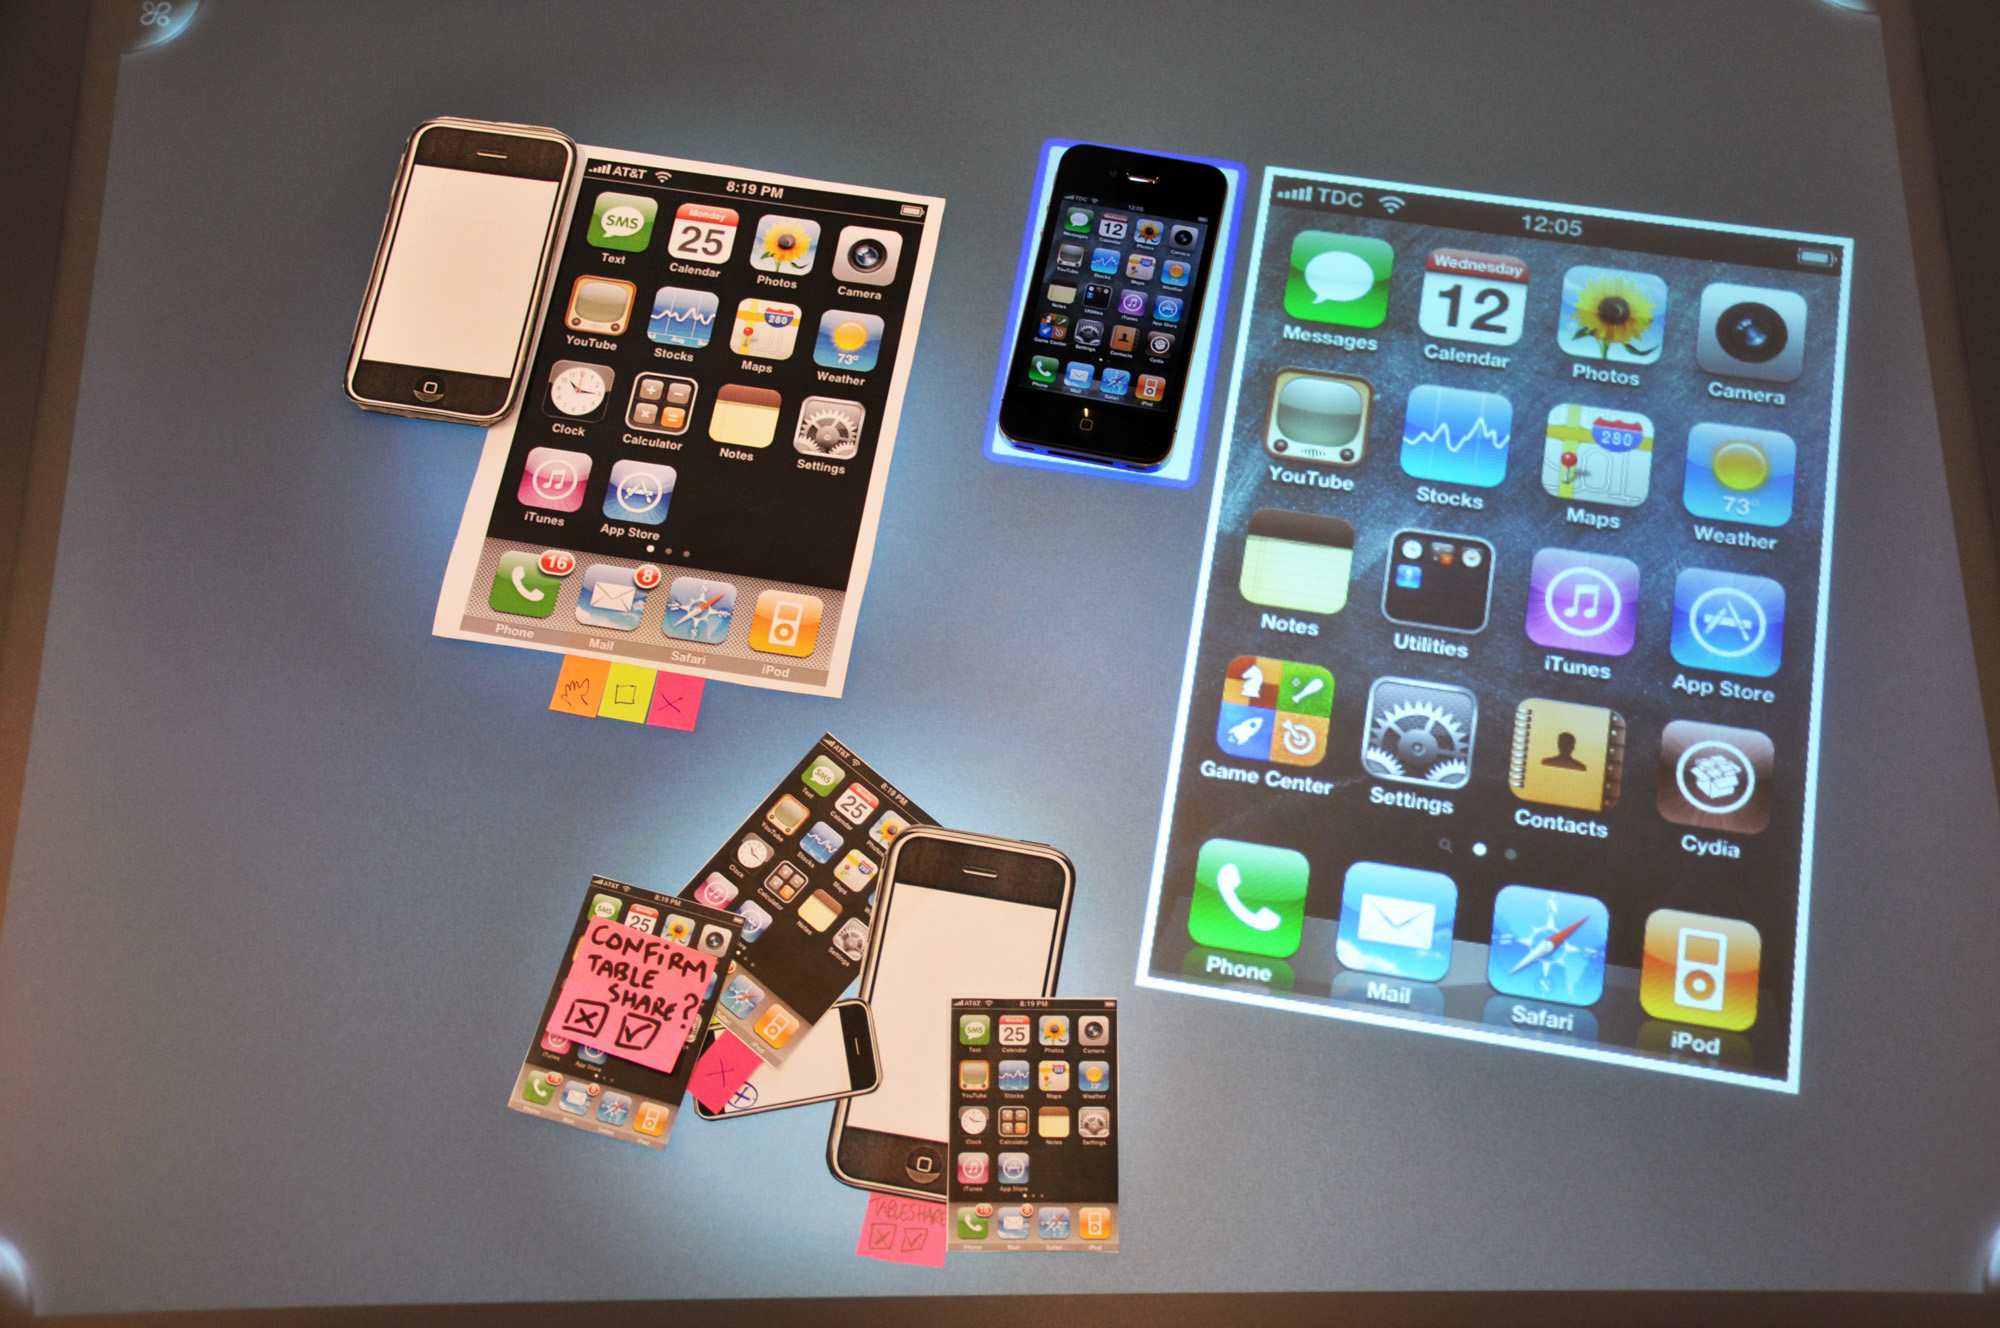
\includegraphics[width=0.8\textwidth]{images/paperprot2}
%\end{figure}

%\begin{figure}[h!]
%  \caption{Low fidelity prototypes.}
%  \centering
%    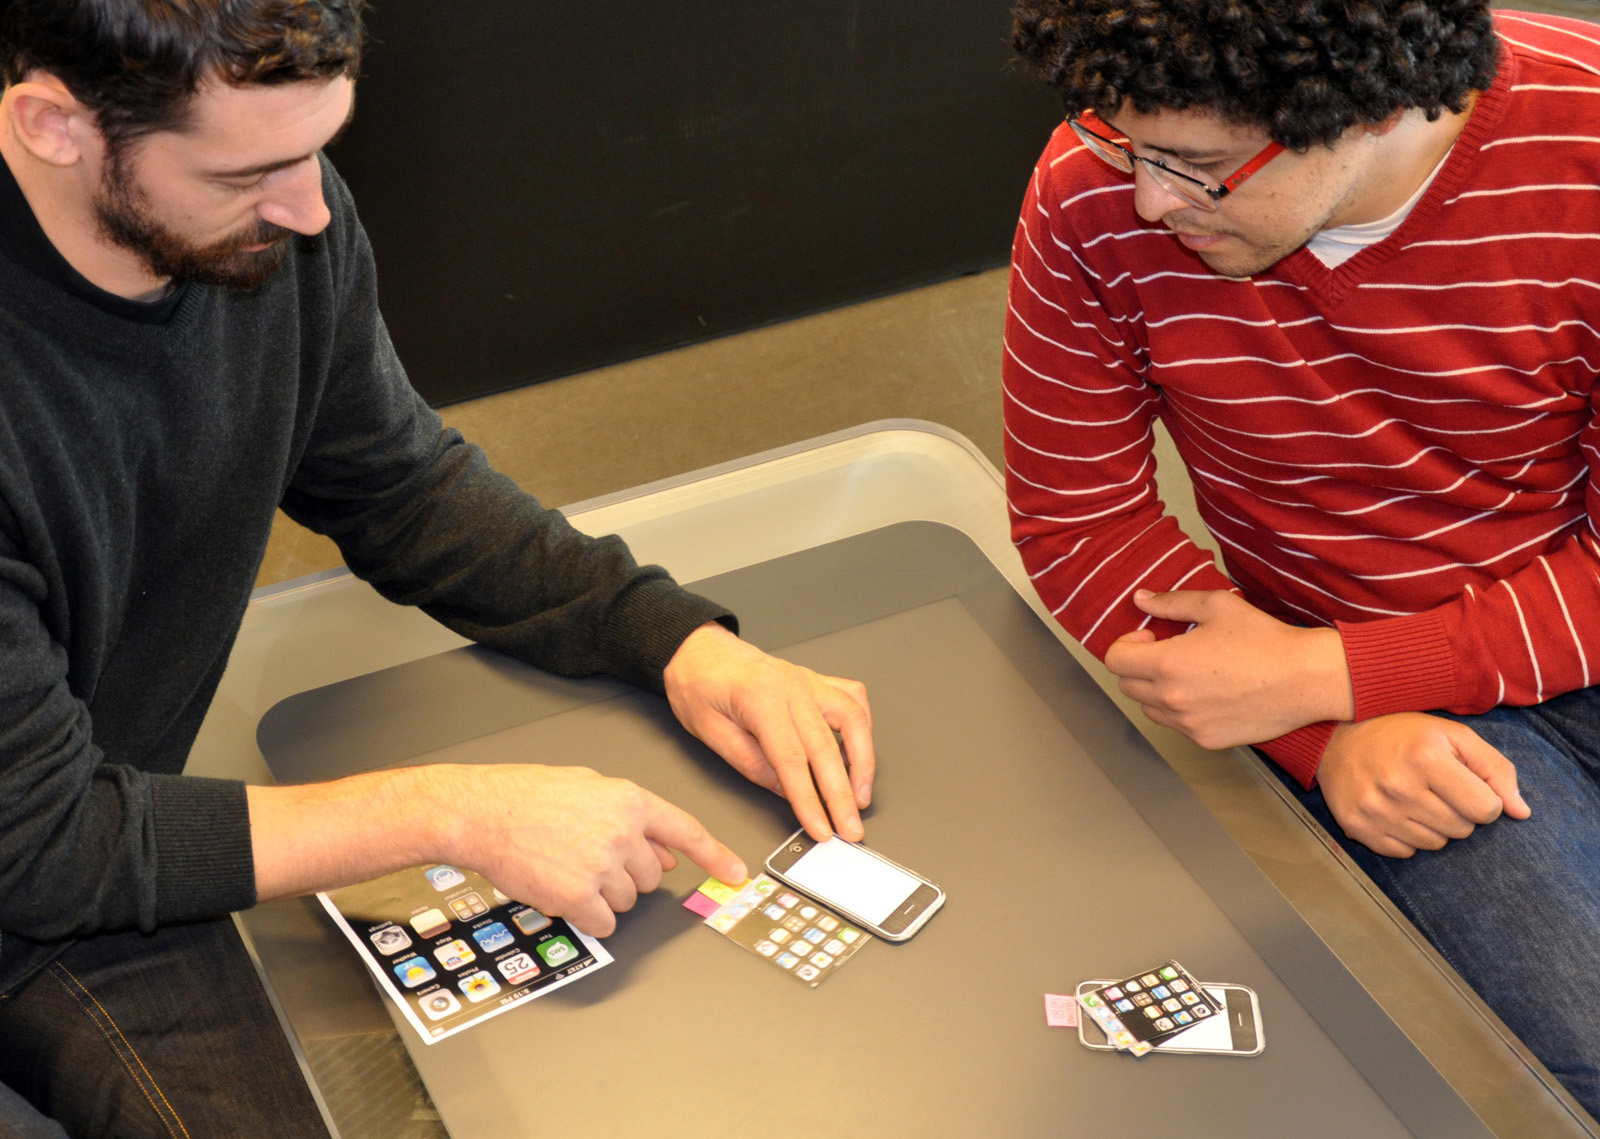
\includegraphics[width=0.8\textwidth]{images/paperprot3}
%\end{figure}

\subsection{Defining interaction stragegies}
\label{sec:strategies}

To support the interaction design process, the concepts of \emph{actions} and \emph{commands} are used.
They are inspired by the work done by Wobbrock et al. on hand gestures for interactive surfaces, \citep{Wobbrock:2009:gestures}.

Human computer interaction can be modeled as a simple cause-effect relationship.
The user wishes the computer to execute a command.
To achieve that, he/she performs an action to provide input.
In the case of a touch-based interactive surface, the action is typically a hand gesture.
The action is the cause, the command is the effect, and together they form a single interaction between user and machine.

\subsubsection{Commands}

The following six basic commands are identified as interaction primitives for the surface UI.

\begin{enumerate}
\item{\emph{Dragging} the application window across the interactive surface.}
\item{\emph{Rotating} the application window across the interactive surface.}
\item{\emph{Resizing} the application window across the interactive surface.}
\item{\emph{Minimizing} the application window, making it possible to restore it easily.}
\item{\emph{Hiding} the content of the application window.}
\item{\emph{Exiting} the application, thus closing the application window.}
\end{enumerate}

It is also agreed that the surface UI should offer an implementation for any supplementary command that is controlled by a physical button on the personal device.

\subsubsection{Actions}


\begin{figure}[ht]
\begin{minipage}[b]{0.5\linewidth}
\centering
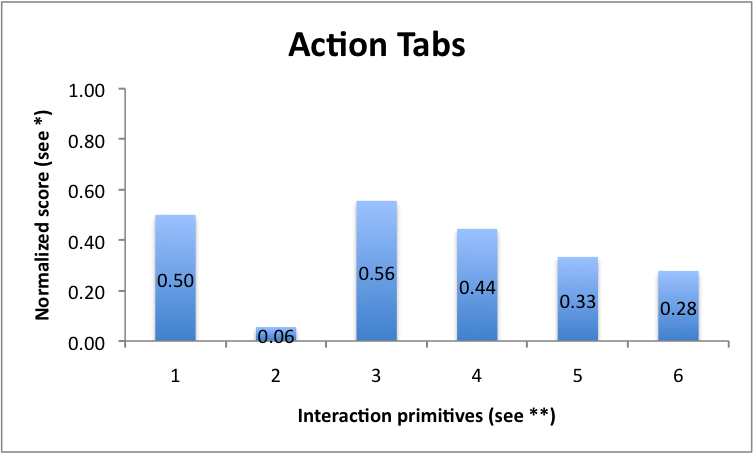
\includegraphics[width=0.8\linewidth]{images/strat1}
\caption{action tabs prototype}
\label{fig:strat1}
\end{minipage}
\hspace{0.5cm}
\begin{minipage}[b]{0.5\linewidth}
\centering
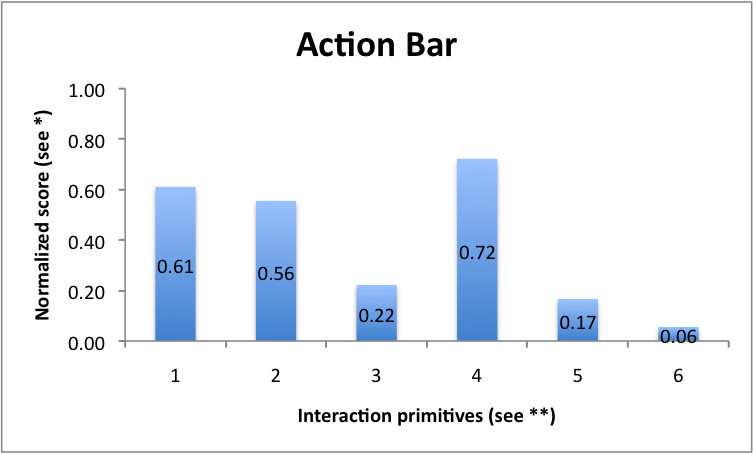
\includegraphics[width=0.8\linewidth]{images/strat2}
\caption{action bar prototype}
\label{fig:strat2}
\end{minipage}
\hfill\\
\begin{minipage}[b]{0.5\linewidth}
\centering
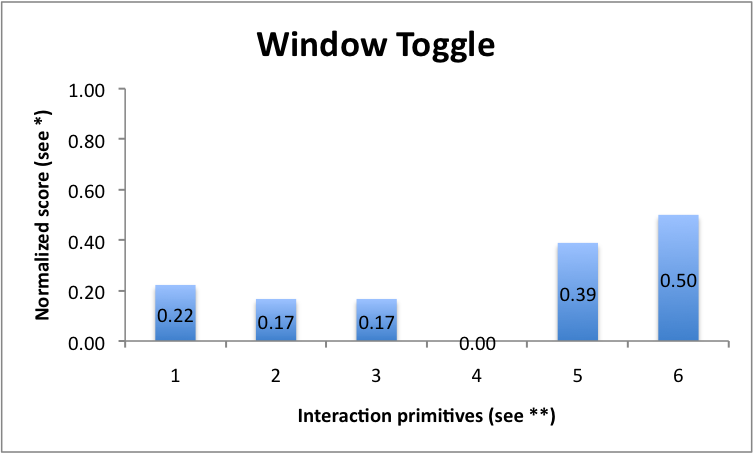
\includegraphics[width=0.8\linewidth]{images/strat3}
\caption{active border prototype}
\label{fig:strat3}
\end{minipage}
\hspace{0.5cm}
\begin{minipage}[b]{0.5\linewidth}
\centering
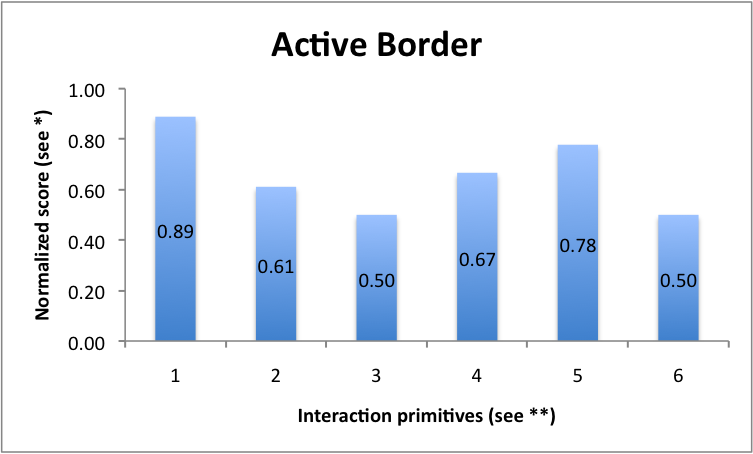
\includegraphics[width=0.8\linewidth]{images/strat4}
\caption{active corners prototype}
\label{fig:strat4}
\end{minipage}
\end{figure}

Various interaction techniques can be used to invoke application level commands, as shown in figures~\ref{fig:strat1} to \ref{fig:strat4}.
Working with paper prototypes to generate ideas lead to the definition of a set of five interaction strategies.
Each strategy can be consistently implemented for each previously defined command.
There is a sixth category, that regroups design suggestions that are not part of a consistent strategy.

\begin{enumerate}
\item{\emph{Action Tabs} are traditional buttons/tabs that implement functionalities.}
\item{The \emph{Action Bar} can be compared to a virtual touchpad, it includes a manipulation area and buttons.}
\item{\emph{Window Toggle} refers to using a switch to toggle the window between inactive and active states. In its inactive state, the window is made manipulable as a common digital picture.}
\item{The \emph{Active Border} is a digital frame around the application window used for manipulation.}
\item{\emph{Active Corners} is a strategy similar to Active Border, with the difference that the border's corners implement specific functionalities.}
\item{\emph{Other} regroups suggestions that do not fit with any specific strategy.}
\end{enumerate}

\section{Preliminary usability study}

In order to design an interactive system that is both usable and engaging, it is important to keep the process human-centred.
This can be done by taking a participatory approach, where users explore and evaluate ideas.
This study was run with this goal in mind.
It is based on an experiment where users engage with low fidelity prototypes of the system, and are asked to evaluate the interaction strategies that are defined in section~\ref{sec:strategies}.

\subsection{Method}	

\subsubsection{Parameters}

The parameters of the experiment are the commands, referred to as \emph{interaction primitives}, and the actions, referred to as \emph{interaction strategies}, defined in section~\ref{sec:strategies}.
The six interaction primitives represent each a system feature that is deemed critical to the overall design.
For each primitive, there are six interaction strategies.
The aim of the study is to have real users compare and evaluate those strategies, and to determine which ones are best fitted for each primitive.

\begin{figure}[htb]
  \centering
    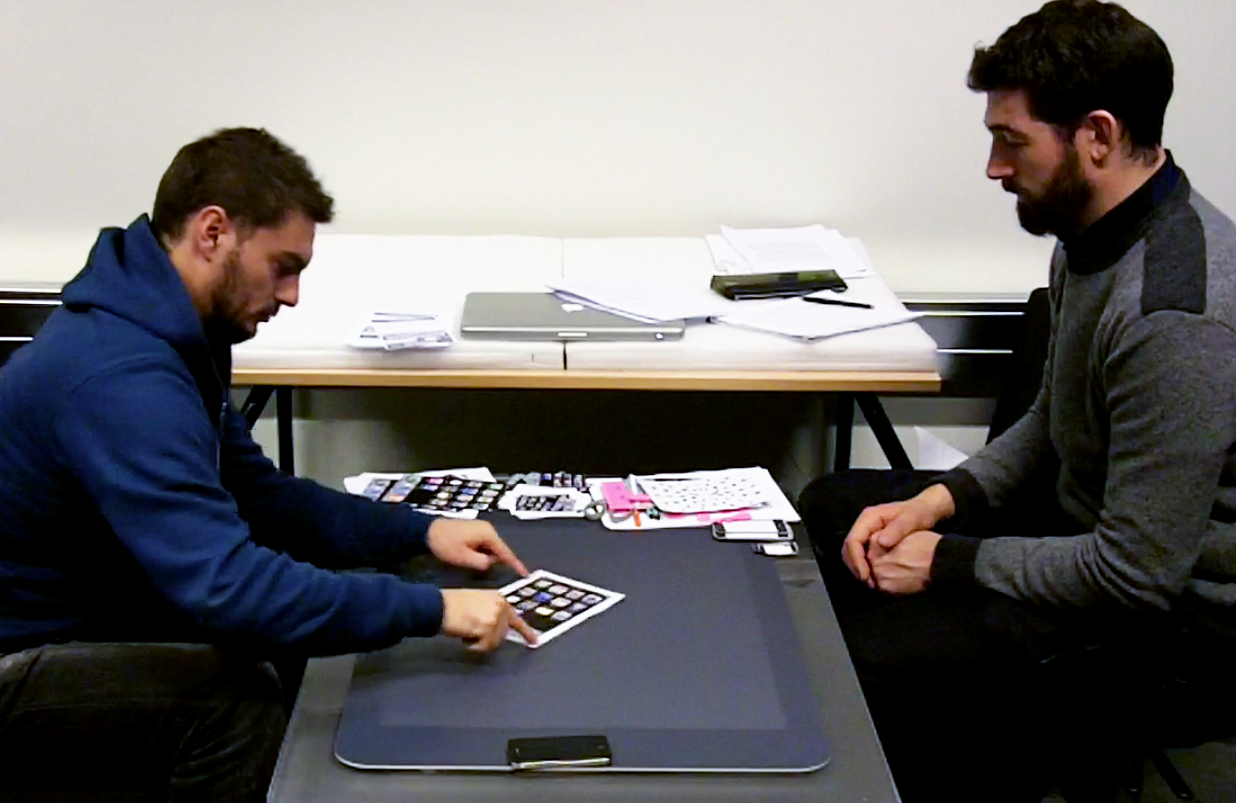
\includegraphics[width=0.8\textwidth]{images/studyScreenshot}
  \caption{Participant and designer during an experiment session.}
  \label{studyScreenshot}
\end{figure}

\subsubsection{Experiment}

Twelve participants were recruited on a voluntary basis.
An experiment session involves one participant and one designer.
The participant sits next to the Microsoft Surface tabletop \citep{ms}, and is presented with an iPhone \citep{iphone}, but both devices are off.
On the tabletop are paper prototypes, that are to be used as representations of UI elements throughout the session.
The designer leads the experiment by reading instructions from a script (included in appendix~\ref{app:study}) and answering the participant's questions.
\hfill\\\\
During the introduction phase, the following things are explained to the participant:
\begin{itemize}
\item the purpose of the study
\item the purpose of the TIDE application
\item the tasks that the participant will perform
\item the principles of working with paper prototypes
\end{itemize}
\hfill\\
During the main experiment, the user is asked to perform a task using the prototyped application.
The task is to write an email, and it requires the user to go through six phases.
Each phase is dedicated to an interaction primitive, and they have the same structure, which is as follows:
\begin{enumerate}
\item the primitive is explained to the participant in terms of a command to the application
\item the user is asked to suggest an action that he/she would perform to obtain the desired effect, and to demonstrate the action using the prototypes
\item the designer gives three action suggestions, the user is asked to demonstrate the actions, then rank them by order of preference.
\end{enumerate}

There is a seventh phase focusing on the pairing procedure.
This phase occurs first and is meant as an example to the participant, describing the common structure.
At the end of this phase, a slide animation is used to describe all six primitives to the user.

For each command, there are six possible actions.
However, it was decided that asking a user to choose between six choices would be overwhelming.
Therefore the volunteers are split into 2 groups, each evaluating a subset of the interaction strategies.
The repartition is shown in table~\ref{groups}.

\begin{figure}[htb]
  \centering
    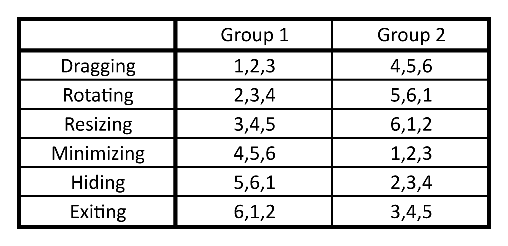
\includegraphics[scale=1]{images/groups}
  \caption{The repartition of the evaluated interaction strategies between the two groups of participants. The strategies are 1)~Action Tabs 2)~Action Bar 3)~Window Toggle 4)~Active Border 5)~Active Corners 6)~Other.}
  \label{groups}
\end{figure}

%Figure \ref{studyScreenshot} shows a typical experiment session.

\subsection{Results}

Participant answers were gathered by the designer in a form such as the one included in appendix~\ref{app:studyForm}.
The form is a matrix where an entry corresponds to a pair (primitive,strategy).
Those entries contains the position from 1 (highest) to 3 (lowest), that was given by the user for using the suggested strategy for implementing the primitive.
After processing all answers, each entry contains 6 positions.
In order to obtain a numeric score for each entry, a weighted average was calculated, giving a weight of 3 to a first position, a weight of 1 to a second position, and a weight of 0 to a third position.
Finally, the results were normalized to a [0-1] interval, where a 1 signifies that the entry was awarded a first position by all participants, and a 0 signifies that all participants ranked this entry third.
Figure~\ref{resultMatrix} summarizes the normalized scores, with colored cells containing values above 0.6.
This is considered a superior score, because it can only be obtained if half of the participants awarded the first position.
The same results are presented in the form of charts in figure~\ref{primitives}.

\begin{figure}[htb]
  \centering
    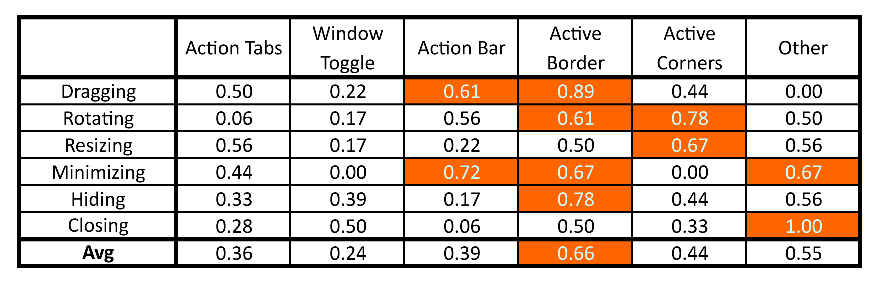
\includegraphics[scale=1]{images/resultMatrix}
  \caption{Normalized weighted average of the ranks given to each pair (primitive, strategy).}
  \label{resultMatrix}
\end{figure}

\begin{figure}[h!]
  \centering
    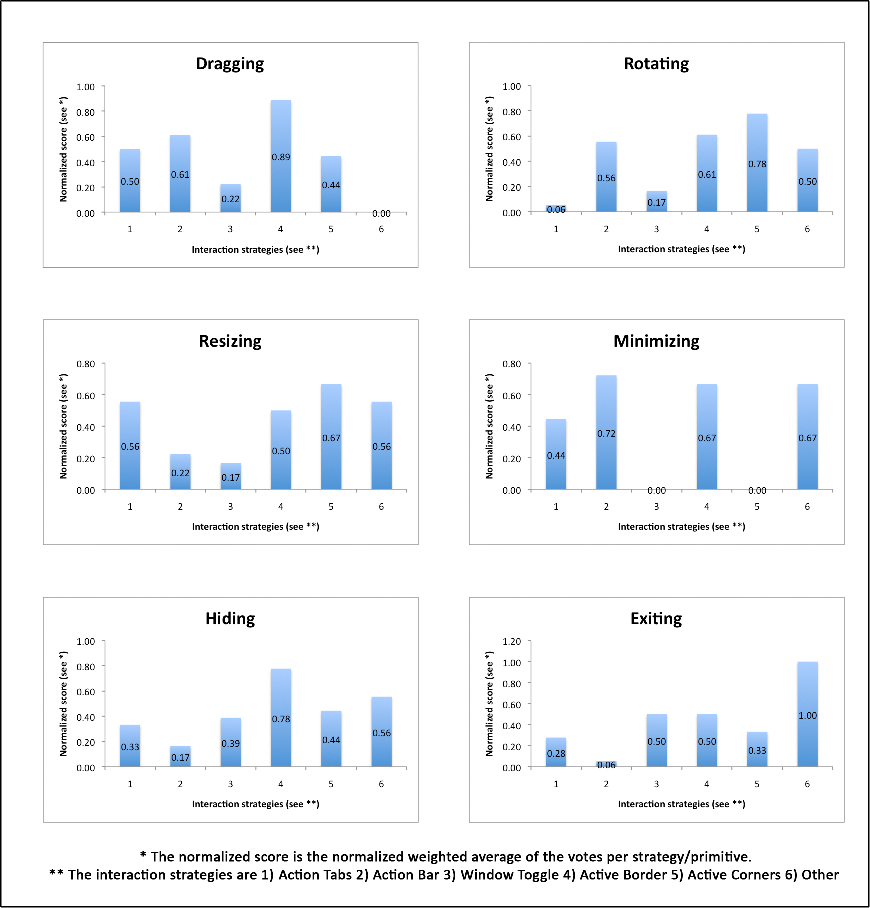
\includegraphics[width=1\textwidth]{images/primHistog}
    \caption{The score of the different interaction strategies for each primitive.}
	\label{primitives}    
\end{figure}

\subsubsection{Analysis}

It is possible to divide the primitives into two groups.
The first half -dragging, rotating, resizing- have a concrete visual signification, where the second half - minimizing, hiding, exiting- are more abstract.

For the first three primitives, there is a strong coherence in the choice of the participants.
The favored strategies are the active border, the action bar and active corners.
All three require the user to interact with an area directly around the window in order to manipulate it and modify its position, orientation or size.
This interaction strategy is similar to the current standard for manipulating pictures on interactive screens, with the difference that in the case of the display extension, the window containing the remote UI is logically avoided because of its role as IO bridge between the tabletop and the personal device.

For the last three primitives, the action bar and active border continue to score high, even though there is no apparent relation between the visual aspect of the strategy and the effect implied by the command.
To understand this, it is necessary to look at the relevant entries in more detail.
The favored strategies for minimizing were double tapping on the action bar and double tapping on the active border.
For hiding, the favored strategy was double tapping on the active border.
It is thus obvious that it is the double tap that participants have a preference for, possibly because it is a common technique in many other application contexts, as well as a quick and easy one.

It is not possible to analyze the scores of the sixth interaction strategy as a whole, as it does not represent a consistent strategy, but more a patchwork of various implementation suggestions.
Those suggestions were chosen because of their originality and interest, and are listed here:
\begin{enumerate}
\item Drag by holding a finger on a specific tab, and using another finger to tap a destination target to move the window to.
\item Rotate by performing a one finger dragging gesture on a corner of the window.
\item Resize by pulling the window apart with both whole hands.
\item Minimize by dragging the window to the bottom of the surface.
\item Hide by placing and holding a full hand on the window.
\item Exit by dragging the window to a specific location on the surface.
\end{enumerate}
Suggestions 4 and 6 are similar, and they are the only ones that scored above 0.6.
This suggests that moving the window off screen is a natural way to remove focus from the application.
It is interesting to see how this correlates with the open suggestion analysis below.

\subsubsection{Open suggestion analysis}

The open suggestions were multiple and heterogeneous, but further analysis showed a definite tendency in three situations.

In the case of dragging, half of the participants suggested using one or more fingers to touch inside the window containing the remote UI, and perform a drag gesture.
This is interesting, because it is an obvious conflict for the developer, i.e.\ any touch inside the window is forwarded to the remote UI, and can therefore not be interpreted as a surface UI manipulation.
It must be noted that dragging was the first primitive, and it can therefore be assumed that the participants did not yet have a full understanding of the remote UI concept.
However, this result shows well that the ideal goal would be to design an interactive system whose UI could interpret the intention of the user.

In the case of resizing, 8 out of 12 participants suggested grabbing the sides of the window with 2 fingers, and pulling the window apart to enlarge it.
This shows that the gesture is very intuitive, and that a good usability would require implementing this interaction technique.

The third consensus was for minimizing, where 7 out of 12 participants suggested dragging the window offscreen (or to a specific location on the surface edge).
The same suggestion reoccurred for the primitives hiding and exiting, though with less decisiveness.
Once again, it shows that the gesture is an intuitive one.
Moreover, there is a direct parallel between removing a real piece of paper from the center of a table, and the act of minimizing, hiding or exiting the display extension application.
Moving the application out of focus seems like a good solution, and using a simple dragging gesture is a natural way of doing it.

%\subsubsection{Dragging}
%
%\subsubsection{Rotating}
%
%\subsubsection{Resizing}
%
%\subsubsection{Minimizing}
%
%\subsubsection{Hiding}
%
%\subsubsection{Exiting}

\section{Design Decisions}

The usability study provided precious input from potential users of the system, and this input supported the designer's views that in order to build a successful system, the focus should be on usability and intuition.
In this context, intuitive interaction means that the user should be able to learn the system through free exploration, all the time guessing and discovering functionalities.
To allow this phenomenon, the implementation should focus on three things.
First, it should be coherent. If the features are consistent, the user will be able to derive one from the other.
Second, common interaction techniques should be used, such as the picture manipulation gestures (drag, pinch, rotate) that are already successful on touch-based interactive screens.
Third, the implementation should refer to the table metaphor when possible, using the user's familiarity with normal table objects to hint at specific features.\\
\hfill\\
The implementation choices are as follows:
\begin{itemize}
\item Dragging, rotating and resizing are done by manipulating an active border that frames the window. The active border has the visual appearance of the body of the physical device.
\item When the window is dragged off an edge of the table, the application is minimized. Minimizing can also be done by double tapping the active border.
\item In its minimized state, the application appears as an icon on the tabletop. This icon can be moved around, restored, or closed.
\item On closing the application, the user will be prompted to confirm exiting the application.
\item Exiting can also be done by dragging the window to a corner of the tabletop, or by pressing and holding one finger on the active border.
\item Hiding is achieved by minimizing the application. Minimizing is therefore also implemented as a result of holding a whole hand over the window.
\item When reduced under a certain threshold, the application is minimized. Similarly when enlarged above a certain size, it is maximized to a fullscreen mode. To escape the fullscreen mode, buttons are implemented in the corners of the tabletop.
\item the buttons present on the physical device are a logical part of the active border, and their functions are implemented accordingly.
\end{itemize}
\hfill\\
In most software applications, there exists two ways to activate the same command.
The advantage is that one implementation can be made to be easy to discover, while the other is more obscure, but a faster or easier interaction.
The best example of this are keyboard shortcuts. They can not be guessed by the novice user, but they are used by the expert user for their efficiency.
Similarly, the display extension can be minimized easily and quickly by double tapping the active border, but the novice user can easily discover the feature by simply dragging the window off screen.
